%%%%%%%%%%%%%%%%%%%%%%%%%%%%%%%%%%%%%%%%%
% University/School Laboratory Report
% LaTeX Template
% Version 3.1 (25/3/14)
%
% This template has been downloaded from:
% http://www.LaTeXTemplates.com
%
% Original author:
% Linux and Unix Users Group at Virginia Tech Wiki 
% (https://vtluug.org/wiki/Example_LaTeX_chem_lab_report)
%
% License:
% CC BY-NC-SA 3.0 (http://creativecommons.org/licenses/by-nc-sa/3.0/)
%
%%%%%%%%%%%%%%%%%%%%%%%%%%%%%%%%%%%%%%%%%

%----------------------------------------------------------------------------------------
%	PACKAGES AND DOCUMENT CONFIGURATIONS
%----------------------------------------------------------------------------------------

\documentclass{article}

%\usepackage[version=3]{mhchem} % Package for chemical equation typesetting
%\usepackage{siunitx} % Provides the \SI{}{} and \si{} command for typesetting SI units
\usepackage{graphicx} % Required for the inclusion of images
\usepackage{natbib} % Required to change bibliography style to APA
\usepackage{amsmath} % Required for some math elements 
\usepackage{amssymb}

\def\deriv#1#2{\frac{d #1}{d #2}}
\def\pp#1#2{\frac{\partial #1}{\partial #2}}

\setlength\parindent{0pt} % Removes all indentation from paragraphs

\renewcommand{\labelenumi}{\alph{enumi}.} % Make numbering in the enumerate environment by letter rather than number (e.g. section 6)

%\usepackage{times} % Uncomment to use the Times New Roman font

%----------------------------------------------------------------------------------------
%	DOCUMENT INFORMATION
%----------------------------------------------------------------------------------------

\title{Simulation of Moving Boundaries: Immersed Boundary and Arbitrary Lagrangian-Eulerian Methods} % Title

\author{A. Cody \textsc{Nunno} and Bruce A. \textsc{Perry}} % Author name

\date{\today} % Date for the report

\begin{document}

\maketitle % Insert the title, author and date


% If you wish to include an abstract, uncomment the lines below
\begin{abstract}
  In the field of computational fluid dynamics (CFD), most algorithms are developed for use in reference frames where the system boundaries are stationary.  Often, however, moving geometries, such as that of a cylindrical piston, must be considered in order to make predictions regarding real systems.  With that in mind, a set of numerical experiments will be performed on a 2D piston geometry with an advancing, receding, or reciprocating boundary.  To address the changing computational domain, two meshing methods will be implemented and compared: the Arbitrary Lagrangian-Eulerian (ALE) method and the Immersed Boundary (IB) method.  ALE uses a moving grid to maintain accuracy and resolution as the geometry of a system changes.  The IB method uses a stationary mesh but requires the addition of a source term to the governing equations near to enforce the boundary conditions when the boundary does not align with the mesh. The advantages and disadvantages of the two methods with regards to simplicity, cost, stability, and accuracy will be compared.
\end{abstract}

%----------------------------------------------------------------------------------------
%	SECTION 1
%----------------------------------------------------------------------------------------

\section{Introduction}

Moving boundaries are often a necessary evil in examining real problems.  While many applications of fluid dynamics study problems with consistent boundaries, such as boundary layers or pipe flow, still others require movement of the domain boundaries.  Modern airplane wings shift the shape of the wing to have more advantageous properties for takeoff, flight, landing, etc., which necessitates a change in boundary conditions for the flow around the craft.  In an internal combustion engine, pistons move up and down, changing the size of the volume of interest and boundary conditions.  Such scenarios are very difficult to simulate using CFD with conventional boundary conditions.  To this end, other methods have been developed to satisfy these scenarios.

 
%----------------------------------------------------------------------------------------
%	SECTION 2
%----------------------------------------------------------------------------------------

\section{Background}

\subsection{ALE}

The first method to be discussed in this work is the Arbitrary Lagrangian-Eulerian, or ALE, method, which uses a moving grid to accomplish the change in the control volume of interest.  In most fluid dynamics textbooks, fluids are typically examined in two different frames: Eulerian, which examines the flow by focusing on a fixed space as fluid passes through, and Lagrangian, which follows the flow through space as it moves.  Typically, CFD solves its given problem on an Eulerian grid; this simplifies the method of solution by maintaining a consistent grid, since, especially in flows which are turbulent, or would otherwise require a grid with irregular remeshing.  These two frames are typically related to one another through the material derivative, given by:
\begin{equation}
  \frac{DF}{Dt} = \deriv{F}{t} + u \cdot \nabla F
\end{equation}
where F is merely some function in the domain.  This allows us to relate any quantity in the Eulerian frame with a kinematical description linked to the moving particle.  

A similar technique can be applied to a moving grid.  There is no particular reason that the moving frame must be attached to the particle, except that it is a useful descriptor.  In a CFD simulation, the grid is also a convenient frame; however, the grid is typically also unmoving.  In ALE, there is propagation of the grid according to the boundary conditions of the problem, which gives meaning to the idea of tracking the grid.  In this frame, we can define a velocity which is relative to the grid:
\begin{equation}
  c = u - \hat{u}
\end{equation}
where $\hat{u}$ is the propagation velocity of the grid.  This term, along with the same logic which lead us to the material derivative, allows us to write an expression for the material derivative using quantities in the grid reference frame:
\begin{equation}
  \frac{DF}{Dt} = \frac{\eth F}{\eth t} + c \cdot \nabla F
\end{equation}
where $\frac{\eth F}{\eth t}$ is the derivative in the frame of the grid.  It is essentially the same, but now the material derivative is taken in the frame of the moving grid.  This substitution is required in the equations of motion for the Eulerian $\deriv{F}{t}$ so as to avoid needing to perform inaccurate operations to advance the simulation in time.  In our three governing equations:
\begin{equation}
  \frac{\eth \rho}{\eth t} + c_j \pp{\rho}{x_j} + \rho \pp{u_j}{x_j}
\end{equation}
\begin{equation}
  \frac{\eth \rho u_i}{\eth t} + c_j \pp{\rho u_i}{x_j} + (\rho u_i)\pp{u_j}{x_j} = - \pp{p}{x_i} + \pp{\tau_{ij}}{x_j}
\end{equation}
\begin{equation}
  \frac{\eth \rho e_t}{\eth t} + c_j \pp{\rho e_t}{x_j} + (\rho e_t)\pp{u_j}{x_j} = - \pp{p u_j}{x_j} + \pp{\tau_{ij} u_j}{x_j}  - \pp{q_j}{x_j}
\end{equation}

ALE is a very popular method for fluid dynamics simulations which involve a shifting grid, especially those which involve fluid structure interactions.  

\subsection{Immersed Boundary}


%----------------------------------------------------------------------------------------
%	SECTION 3
%----------------------------------------------------------------------------------------

\section{Method of Solution}

\subsection{ALE}

Solving the ALE equations necessitated a compressible flow solver, as the particular problem considered in this work involves significant compression.  Additionally, the implementation in the compressible flow solver was found to be somewhat easier.  To solve these equations, a simple set of finite difference equations have been implemented.  The time integration is done using explicit Euler, and the derivatives of quantities are found using second order central difference from cell corner to corner.  The only exception is the fluxes, which are taken and stored at the midpoints of the cell sides, which is done to ensure that when the derivative of these fluxes are taken, it resembles a second order central difference.  To illustrate, the continuity, momentum, and energy equations, as discretized, are repeated below:
\begin{equation}
  \frac{\rho^{n+1}_{i,j} - \rho^{n}_{i,j}}{\Delta t} = - u^{n}_{i,j} \frac{\rho^{n}_{i+1,j}-\rho^{n}_{i-1,j}}{2\Delta x} - c^{n}_{i,j} \frac{\rho^{n}_{i,j+1}-\rho^{n}_{i,j-1}}{2\Delta y} + \rho^{n}_{i,j} \left(\frac{u^{n}_{i+1,j}-u^{n}_{i-1,j}}{2\Delta x} + \frac{u^{n}_{i,j+1}-u^{n}_{i,j-1}}{2\Delta y}\right)
\end{equation}
\begin{equation}
  \frac{(\rho u)^{n+1}_{i,j} - (\rho u)^{n}_{i,j}}{\Delta t} = - u^{n}_{i,j} \frac{(\rho u)^{n}_{i+1,j}-(\rho u)^{n}_{i-1,j}}{2\Delta x} - c^{n}_{i,j} \frac{(\rho u)^{n}_{i,j+1}-(\rho u)^{n}_{i,j-1}}{2\Delta y} + (\rho u)^{n}_{i,j} \left(\frac{u^{n}_{i+1,j}-u^{n}_{i-1,j}}{2\Delta x} + \frac{v^{n}_{i,j+1}-v^{n}_{i,j-1}}{2\Delta y}\right) - \frac{p^{n}_{i+1,j} - p^{n}_{i-1,j}}{2\Delta x} + \frac{(\tau_{xx})^{n}_{i+1/2,j} - (\tau_{xx})^{n}_{i-1/2,j}}{\Delta x} + \frac{(\tau_{yx})^{n}_{i,j+1/2} - (\tau_{yx})^{n}_{i,j-1/2}}{\Delta y}
\end{equation}
\begin{equation}
  \frac{(\rho v)^{n+1}_{i,j} - (\rho v)^{n}_{i,j}}{\Delta t} = - u^{n}_{i,j} \frac{(\rho v)^{n}_{i+1,j}-(\rho v)^{n}_{i-1,j}}{2\Delta x} - c^{n}_{i,j} \frac{(\rho v)^{n}_{i,j+1}-(\rho v)^{n}_{i,j-1}}{2\Delta y} + (\rho v)^{n}_{i,j} \left(\frac{u^{n}_{i+1,j}-u^{n}_{i-1,j}}{2\Delta x} + \frac{v^{n}_{i,j+1}-v^{n}_{i,j-1}}{2\Delta y}\right) - \frac{p^{n}_{i,j+1} - p^{n}_{i,j-1}}{2\Delta y} + \frac{(\tau_{xy})^{n}_{i+1/2,j} - (\tau_{xy})^{n}_{i-1/2,j}}{\Delta x} + \frac{(\tau_{yy})^{n}_{i,j+1/2} - (\tau_{yy})^{n}_{i,j-1/2}}{\Delta y}
\end{equation}
\begin{equation}
  \frac{(\rho e_t)^{n+1}_{i,j} - (\rho e_t)^{n}_{i,j}}{\Delta t} = - u^{n}_{i,j} \frac{(\rho e_t)^{n}_{i+1,j}-(\rho e_t)^{n}_{i-1,j}}{2\Delta x} - c^{n}_{i,j}\frac{(\rho e_t)^{n}_{i,j+1}-(\rho e_t)^{n}_{i,j-1}}{2\Delta y} + (\rho e_t)^{n}_{i,j} \left(\frac{u^{n}_{i+1,j}-u^{n}_{i-1,j}}{2\Delta x} + \frac{v^{n}_{i,j+1}-v^{n}_{i,j-1}}{2\Delta y}\right) - \frac{p^{n}_{i+1,j}u^{n}_{i+1,j} - p^{n}_{i-1,j} u^{n}_{i-1,j}}{2\Delta x} - \frac{p^{n}_{i,j+1} v^{n}_{i,j-1} - p^{n}_{i,j-1} v^{n}_{i,j-1}}{2\Delta y} + \frac{u^{n}_{i+1/2,j}(\tau_{xx})^{n}_{i+1/2,j} - u^{n}_{i-1/2,j} (\tau_{xx})^{n}_{i-1/2,j}}{\Delta x} + \frac{v^{n}_{i,j+1/2} (\tau_{yx})^{n}_{i,j+1/2} - v^{n}_{i,j-1/2} (\tau_{yx})^{n}_{i,j-1/2}}{\Delta y} + \frac{u^{n}_{i+1/2,j} (\tau_{xy})^{n}_{i+1/2,j} - u^{n}_{i-1/2,j}(\tau_{xy})^{n}_{i-1/2,j}}{\Delta x} + \frac{v^{n}_{i,j+1/2} (\tau_{yy})^{n}_{i,j+1/2} - v^{n}_{i,j-1/2} (\tau_{yy})^{n}_{i,j-1/2}}{\Delta y} - \frac{(q_x)^{n}_{i+1/2,j} - (q_x)^{n}_{i-1/2,j}}{\Delta x} - \frac{(q_y)^{n}_{i+1/2,j} - (q_y)^{n}_{i-1/2,j}}{\Delta y}
\end{equation}
Here, $q$ is the heat flux in the given direction from the cell, and $\tau$ is the shear stress of the cell along the appropriate face.  The fluxes of density weighted quantities, $\rho$, $\rho u$, $\rho v$, and $\rho e_t$, can be found using these equations.  Other variables, such as $p$ and $T$, can be found using the definition of energy, or the ideal gas equation:
\begin{equation}
  \rho e_t = \frac{1}{\gamma -1} p + \frac{1}{2} \rho (u^2 + v^2)
\end{equation}
\begin{equation}
  p = \rho R T
\end{equation}
The primary difference between this implementation and the implementation used on project two and elsewhere in this project is that the equations are dimensional so as to make the introduction of the grid velocity conceptually simpler.
\begin{figure}
    \centering
    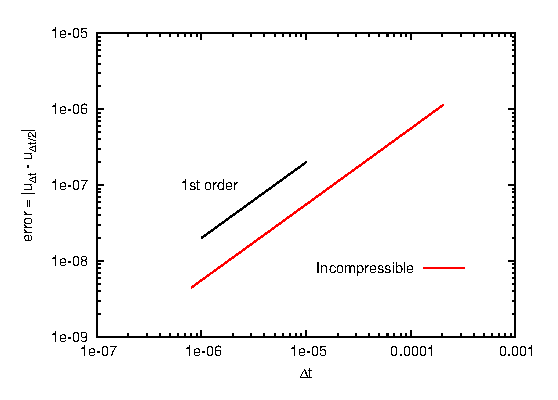
\includegraphics[width=0.7\textwidth]{timeconv.eps}         
    \caption{Time convergence for ALE.}
    \label{fig:timeconv}
  \end{figure}
\begin{figure}
    \centering
    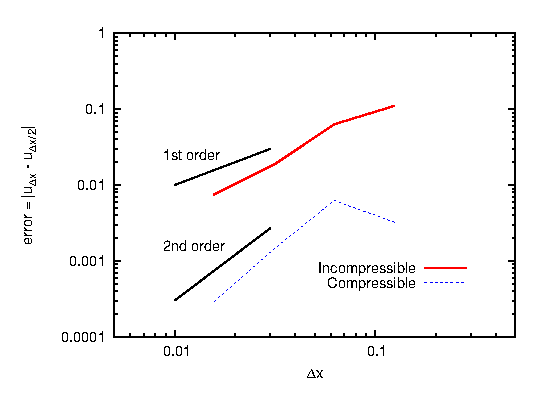
\includegraphics[width=0.7\textwidth]{spaceconv.eps}         
    \caption{Spatial convergence for ALE.}
    \label{fig:spaceconv}
  \end{figure}
As we are continuing to use second order central difference and explicit Euler, convergence should be second order in space and first order in time. (INSERT CONVERGENCE HERE)  The anticipated time convergence is achieved, as can be seen in Figure~\ref{fig:timeconv}.
Because of the shrinking and expanding grid size, it is impossible to get an exact timestep restriction for ALE.  However, using some analogous analysis to fixed grids, we find the stability criterion to be:
\begin{equation}
  a = b
\end{equation}

\begin{figure}
    \centering
    \includegraphics[width=0.7\textwidth]{masscons.eps}         
    \caption{Mass conservation for ALE.}
    \label{fig:masscons}
  \end{figure}
The conservation properties of the ALE solver change fairly significantly over the original solver from the previous project.  This change is necessary, as the change of reference frame requires the separation of the divergence into two components.  It alters the symmetry of the momentum governing equations' summations, which means that they no longer sum to zero over the entire domain.  However, because of the particular problem configuration addressed in this work, neither momentum nor energy conservation can be verified.  Since a moving piston boundary is being considered, work is being done either on or by the system; therefore, the energy and momentum of the system are being directly affected.  We can, however, still establish mass conservation, by summing the densities multiplied by the volume of each cell and the number of cells.  This information is tracked in Figure~\ref{fig:masscons}.  It is evident from the image that mass is not quite fully conserved, though the variation is minimal over a full cycle, less than 1\% of the total.  

\subsection{Immersed Boundary}


%----------------------------------------------------------------------------------------
%	SECTION 4
%----------------------------------------------------------------------------------------

\section{Application: The Moving Piston}

The great advantage of using both of these methods is their ability to handle moving objects within the flow, or objects which move the flow.  To that end, the test of these methods will be an application which is common in the field of fluid dynamics: the flow incuded by a moving piston.  The problem is two dimensional, with a fixed width in x, both dimensionally and non-dimensionally unity, and an advancing and withdrawing piston under two sets of velocity conditions.  In one condition, the piston will be examined with a constant velocity, given by the function:
\begin{equation}
  v_w = 2 (L1-L2) \omega
\end{equation}
where $\omega$ is the frequency of oscillation in cycles per second, though this condition is not truly oscillatory.  This yields a constant velocity withdrawal or expansion based on an initial and final position of the expansion or compression, L1 and L2, respectively.  These conditions do not experience a full cycle, as the high jerk movement of a sudden and rapid shift in speed is neither particularly realistic nor particularly stable.  In the other condition, the velocity is sinusoidal, given by the equation:
\begin{equation}
  v_w = \pi \omega (L2-L1) \sin{2 \pi \omega t}
\end{equation}
These two conditions are matched such that the frequency of oscillation is the same between them, and the resulting cycles should match pace, although not speed.  

To compare between the two different methods presented, some non-dimensional parameters need to be established to maintain commonality in testing.  The piston

\subsection{ALE}



\subsection{Immersed Boundary}


%----------------------------------------------------------------------------------------
%	SECTION 5
%----------------------------------------------------------------------------------------

\section{Conclusions}




%----------------------------------------------------------------------------------------
%	BIBLIOGRAPHY
%----------------------------------------------------------------------------------------

\bibliographystyle{apalike}

\bibliography{finproj}

%----------------------------------------------------------------------------------------


\end{document}
